\newpage
\section{Ergebnisse}
Dieses Kapitel stellt die zentralen Ergebnisse des Projekts vor. 
Zunächst wird der \acs{aas}-Demonstrator der robocell vorgestellt.
Im Anschluss folgt die Analyse des eingesetzten \acs{ki}-Modells sowie die Präsentation der beiden Anwendungsfälle. 
Abschließend werden die eingesetzten Tools und Softwarelösungen evaluiert.

% \newpage
% \begin{figure}[htbp]
%     \centering
%         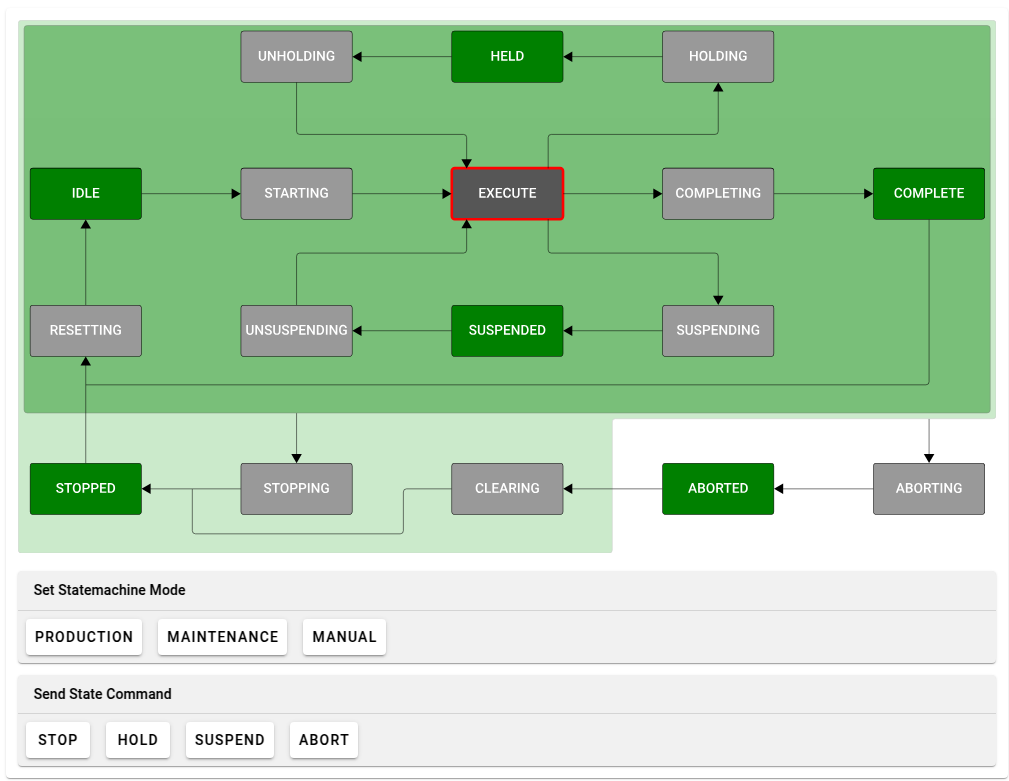
\includegraphics[width=1\textwidth]{Bilder/Ergebnisse/2025-07-23_15-06.png}
    
%     \caption{Sequenzdiagramm zur Aggregation des PCF}
%     \label{fig:SequenzdiagrammPCF}
% \end{figure}



% \begin{figure}[htbp]
%     \centering
%         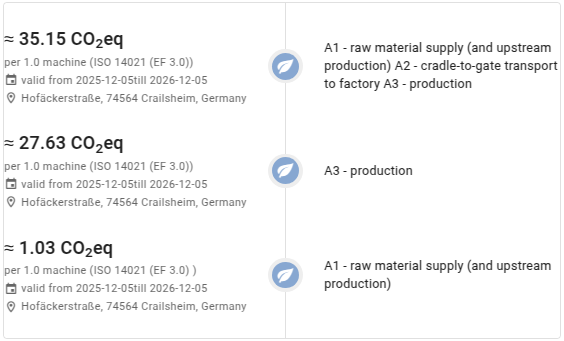
\includegraphics{Bilder/Ergebnisse/DPP/PluginAggregation.png}
    
%     \caption{Sequenzdiagramm zur Aggregation des PCF}
%     \label{fig:SequenzdiagrammPCF}
% \end{figure}
%AAS Demonstrator
\subsection{AAS-Demonstrator für die robocell}
Die statische Mollierung erfolgte ausschließlich mit dem Package Explorer.
Zur Überführung in eine Typ-2-\acs{aas} wurd zu Beginn des Projekts der AASX Server Blazor eingesetzt, der aber relativ schnell durch die Eclipse BaSyx-Plattform abgelöst wurde.

Das Konzept der AAS war neu für groninger
Im folgenden wird die Gesamtarchitektur des Systems aufgezeigt.

Nachfolgende Abbildung zeigt den grundelgenden Aufbau des Systems zur Verwaltung des digitalen Zwillings.
Dieses ist essenziell, da somit erst ein digitaler Zwilling entsteht

\begin{figure}[htbp]
    \centering
        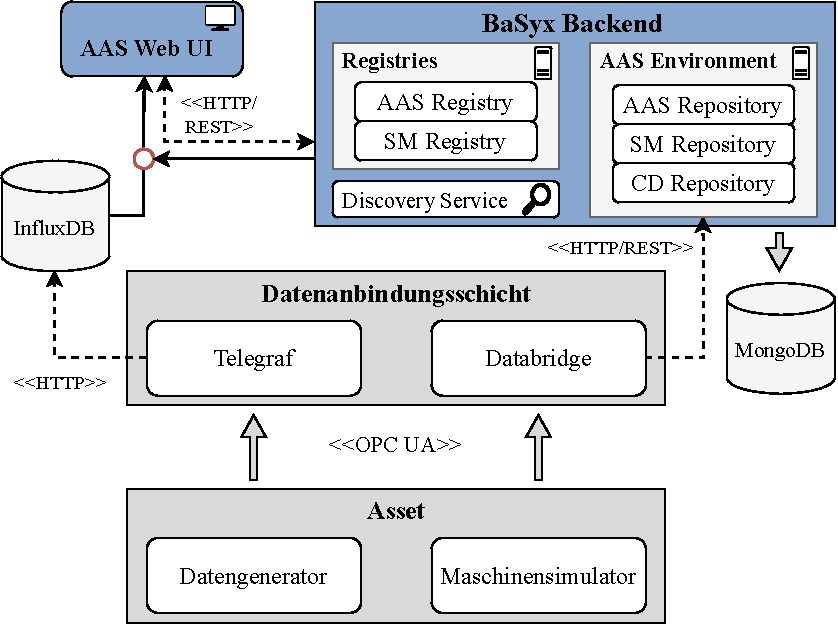
\includegraphics[width=1\textwidth]{Bilder/Ergebnisse/DynamischeDaten/Architektur.pdf}
    
    \caption{Sequenzdiagramm zur Aggregation des PCF}
    \label{fig:SequenzdiagrammPCF}
\end{figure}




\subsubsection{Systemarchitektur}
Die Gesamtarchitektur des Demonstrators basiert vollständig auf containerisierten Komponenten, wodurch eine sklaierbare Struktur entsteht.
Es ist wichtig zu verstehen, ein richtiger digitaler Zwilling entsteht erst durch die Anbindung an das Asset und idealerweise auch
Nachfolgend Gesamtarchitektur.
Alle Kompnonenten als DOcker, BaSyx, Datengeneraot, Machinensimulator auch Docerk aber node.js und OPC UA Server.
Dann Telegraf mit dem die Daten in 
\subsubsection{Statische Submodelle}

\subsubsection{Dynamische Submodelle}

Für die Inegration des Mashcinenstatus wurde die Databridge eingesetzt.
Für Submodell Kontrollkomponente wurde hierfür ein Submodell entworfen, das den aktuellen Zustand der Maschine abbildet.
Dabei stand ein Plugin zur Verfügung das bereits einen solchen Zustandsautomat abbildet.
Allerdings wurde dieses nicht ausfürlich beschrieben, bzw. nur im Rahmne eines Forschungsprojekts von ... vorgestellt.
Darin wird es beschrieben.
Das von denen entwickelte Vue.js Plugin wurde also angepasst.

Dazu wurde eine Logik implementiert, die wenn das Plugin aktiv ist den Maschinesatuts in regelmäßigen Abständen pollt.
Ändert sich dieser so wird der entsprechende Status gesetzt und zudem die OOperatiuonen die ausgeführt werden können.

Die Kontrollkomponenten ermöglicht also theoretisch die Steuerung der Maschine.
Der Maschinensimulator wurde so konfiguriert das wenn der Status geändert wird zum Beispiel drückt ein Nutzer den Stop Button so wird der Zustand der Maschin, wie im Mashcinesimulator abgebildet gestoppt.
Das ist im Sinne eines richtigen digitalen Zwillings wenn das ganze automatisiert wird könnte zum Beispiel der digitale Zwiloing analig Einfluss auf die Maschine nehmen, zum Beispiel wenn Fehler erkannt werden



Der Macshinensimulator simuliert PackML dabei die Werte über OPC UA
Die Databridge holt die jeweiligen Werte

\subsubsection{Herausforderungen bei der Implementierung}

%KI-Modell
\subsection{Evaluation des KI-Modells}
\subsubsection{Bewertung des prototypischen KI-Einsatzes}
\subsubsection{Ausblick: Predictive Maintenance}
\subsubsection{Weiterführende Einsatzmöglichkeiten}

% Digitaler Produktpass
\subsection{Anwendungsfall Digitaler Produktpass}
\subsubsection{Abbildung des PCF}

Die Aggregationslogik ist als eigenständiger, Node.js-basierter Microservice mit einer Web-API implementiert. 
Diese wertet die Komponenten-\acs{aas} aus, berechnet die aggregierten Werte für die zuvor definierten Lebenszyklusphasen und schreibt diese in das \acs{cf}-Submodell der Haupt-AAS der robocell zurück. 
Die Auslösung des Microservice erfolgt über die Schaltfläche im erweiterten Plugin.

Alternativ wäre auch eine clientseitige Berechnung direkt im \acs{cf}-Plugin denkbar. 
In der vorliegenden Umsetzung liegt die gesamte Aggregationslogik jedoch zentral und serverseitig im Microservice. 


Der Ablauf ist in Abbildung \ref{fig:SequenzdiagrammPCF} als Sequenzdiagramm dargestellt.

\newpage
\begin{figure}[htbp]
    \centering
        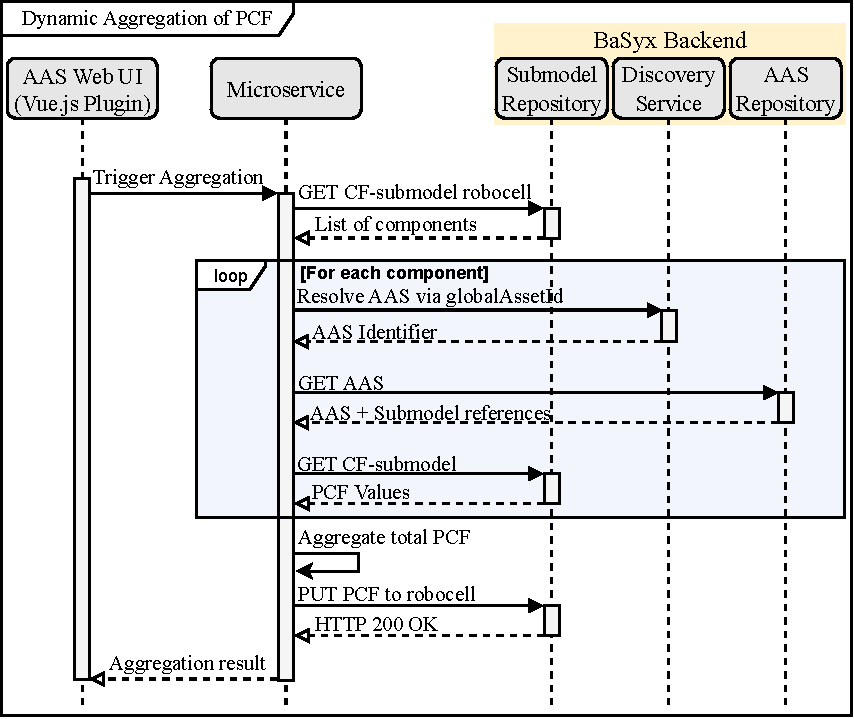
\includegraphics[width=1\textwidth]{Bilder/DPP/PCF_Aggregation_SmallLine.pdf}
    
    \caption{Sequenzdiagramm zur Aggregation des PCF}
    \label{fig:SequenzdiagrammPCF}
\end{figure}

Der Microservice nutzt die \acs{rest}-Schnittstelle des Submodel Repositories der AAS Environment, um zunächst alle in der \acs{aas} der robocell hinterlegten Komponenten auszulesen. 
Mithilfe des Discovery Service werden auf Basis ihrer globalAssetIds die zugehörigen Komponenten-\acs{aas} identifiziert und anschließend vom AAS Repository abgerufen.
Für jede dieser Komponenten wird geprüft, ob ein \acs{cf}-Submodell vorhanden ist. 
Falls dies zutrifft, wird das Submodell ausgelesen und die enthaltenen Werte extrahiert.

Aus den ermittelten Einzelwerten berechnet der Microservice schließlich die aggregierten CO\textsubscript{2}-Äquivalente für die Phasen Produktion, Material sowie Cradle to Gate. 
Die berechneten Werte werden abschließend in das \acs{cf}-Submodell der Haupt-\acs{aas} der robocell geschrieben und stehen dort strukturiert zur Verfügung.

Die beschriebene Lösung ermöglicht es, den \acs{pcf} dynamisch auf Basis der in der Komponentenliste referenzierten Steuerungselemente zu berechnen. 
Auch wenn derzeit nur ausgewählte Komponenten berücksichtigt werden, lässt sich die Liste bei Verfügbarkeit weiterer Komponenten-\acs{aas} unkompliziert erweitern, sodass sukzessive die gesamte Maschine in die Berechnung einbezogen werden kann. 
Perspektivisch lässt sich die Berechnung zudem um weitere Lebenszyklusphasen wie Nutzung oder Entsorgung ergänzen, um eine ganzheitliche Betrachtung von der Herstellung bis zum Lebensende eines Produkts bzw. einer Maschine zu ermöglichen.

\subsubsection{Rollenbasierter Zugriff auf Submodelle}
Eine Möglichkeit, die im \acs{dpp} enthaltenen Informationen einzusehen, bietet die AAS Web UI. 
Ist \acs{rbac} aktiviert, wird der Benutzer beim Aufruf der Oberfläche zur Keycloak-Anmeldeseite weitergeleitet. 
Wie in Abbildung dargestellt, kann der Nutzer sich dort mit Nutzernamen und Passwort anmelden.

\begin{figure}[htbp]
    \centering
        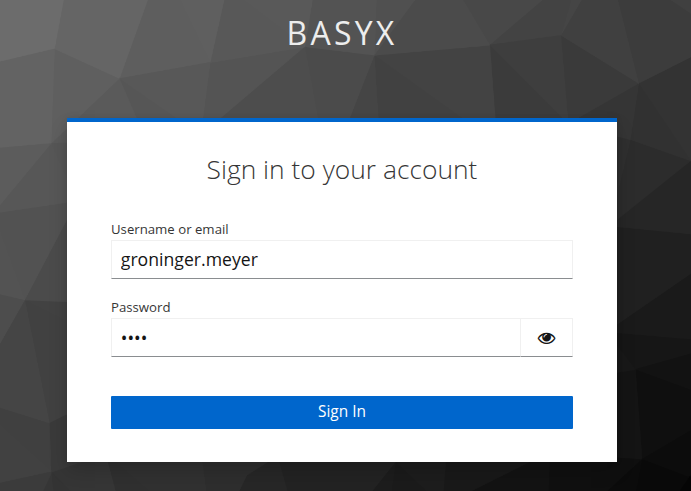
\includegraphics[width=0.7\textwidth]{Bilder/Ergebnisse/DPP/KeycloakAnmeldeSeite.png}
    
    \caption{Keycloak-Anmeldeseite für die AAS Web UI}
    \label{fig:SequenzdiagrammPCF}
\end{figure}

Nach erfolgreicher Authentifizierung erhält der registrierte Client (AAS Web UI) ein Zugriffstoken, das die Rolleninformationen des Nutzers enthält.  
Dieses Token wird im Hintergrund an die angebundenen BaSyx-Komponenten (z.\,B. AAS Environment, Registry) weitergegeben.  
Die Entscheidung über die tatsächliche Zugriffsberechtigung trifft dabei nicht die AAS Web UI, sondern der jeweilige Service, indem er die im Token enthaltenen Rollen gegen die hinterlegten RBAC-Regeln prüft.

+++ Wie ist es wenn nicht alles konfiguriert \\
Beipsiel an Rolle Servgice kann nicht shocladen z.B.\\
 Funkltioniert alles +++\\

Alternativ ist auch ein direkter Zugriff über die \acs{api} möglich, etwa durch technische Clients oder externe Anwendungen.  
In diesem Fall muss das Zugriffstoken aktiv über den Token-Endpunkt des entsprechenden Realms bei Keycloak angefordert und anschließend im \acs{http}-Header der Anfrage übermittelt werden.  
Die Autorisierung erfolgt analog zur Web-Oberfläche durch die jeweiligen BaSyx-Komponenten basierend auf den Rollen im Token und den definierten \acs{rbac}-Konfigurationen.

+++ Mit Postman zeigen +++\\
+++ Für jede Rolle +++\\

+++ Fazit +++ \\

Zeigt dass sich differenzierte Zugriffskontrollen auf Submodell-Ebene technisch realisieren lassen. 
Dies bietet Potenzial für zukünftige Szenarien, bei denen sensible Nachhaltigkeitsdaten nur bestimmten Akteuren entlang der Wertschöpfungskette zugänglich gemacht werden sollen.

\subsection{Anwendungsfall automatisierte Generierung der AAS}
% \subsection{Einsatzmöglichkeiten von KI im Kontext der Verwaltungsschale}
% \subsubsection{Generierung von Verwaltungsschalen}
% \subsubsection{Anomaliererkennung}
% \subsubsection{Weiterführende Einsatzmöglichkeiten}

%Evaluation der eingesetzten Software
\subsection{Evaluierung eingesetzter Tools und Software}
\subsubsection{AASX Package Explorer}
\subsubsection{Eclipse AASX Server}
\subsubsection{BaSyx}
\subsubsection{Mnestix Browser}
Optional davor halt nicht drauf eingeganen\dots